\newpage

\section{Side-Splitter Theorems}
In this activity, we will show that the properties of dilations, which you noticed in a previous activity, can be proven \emph{without} using facts about transversals and parallel lines.  Instead, we use the area formulas for rectangles, triangles, and parallelograms.  
\begin{question}
What must be true about the base and height measurements for these area formulas to be valid? 
\end{question}

\fixnote{Either tilt the following triangle or add another problem with a tilted triangle.}

\begin{prob}
If the area of $\triangle SPR = 5$ square inches and the area of $\triangle QPR = 8$ square inches, then what can you say about $\frac{SR}{RQ}$?  What about $\frac{SR}{SQ}$?  What can you say generally about how these ratios depend upon the areas of the triangles?  
$$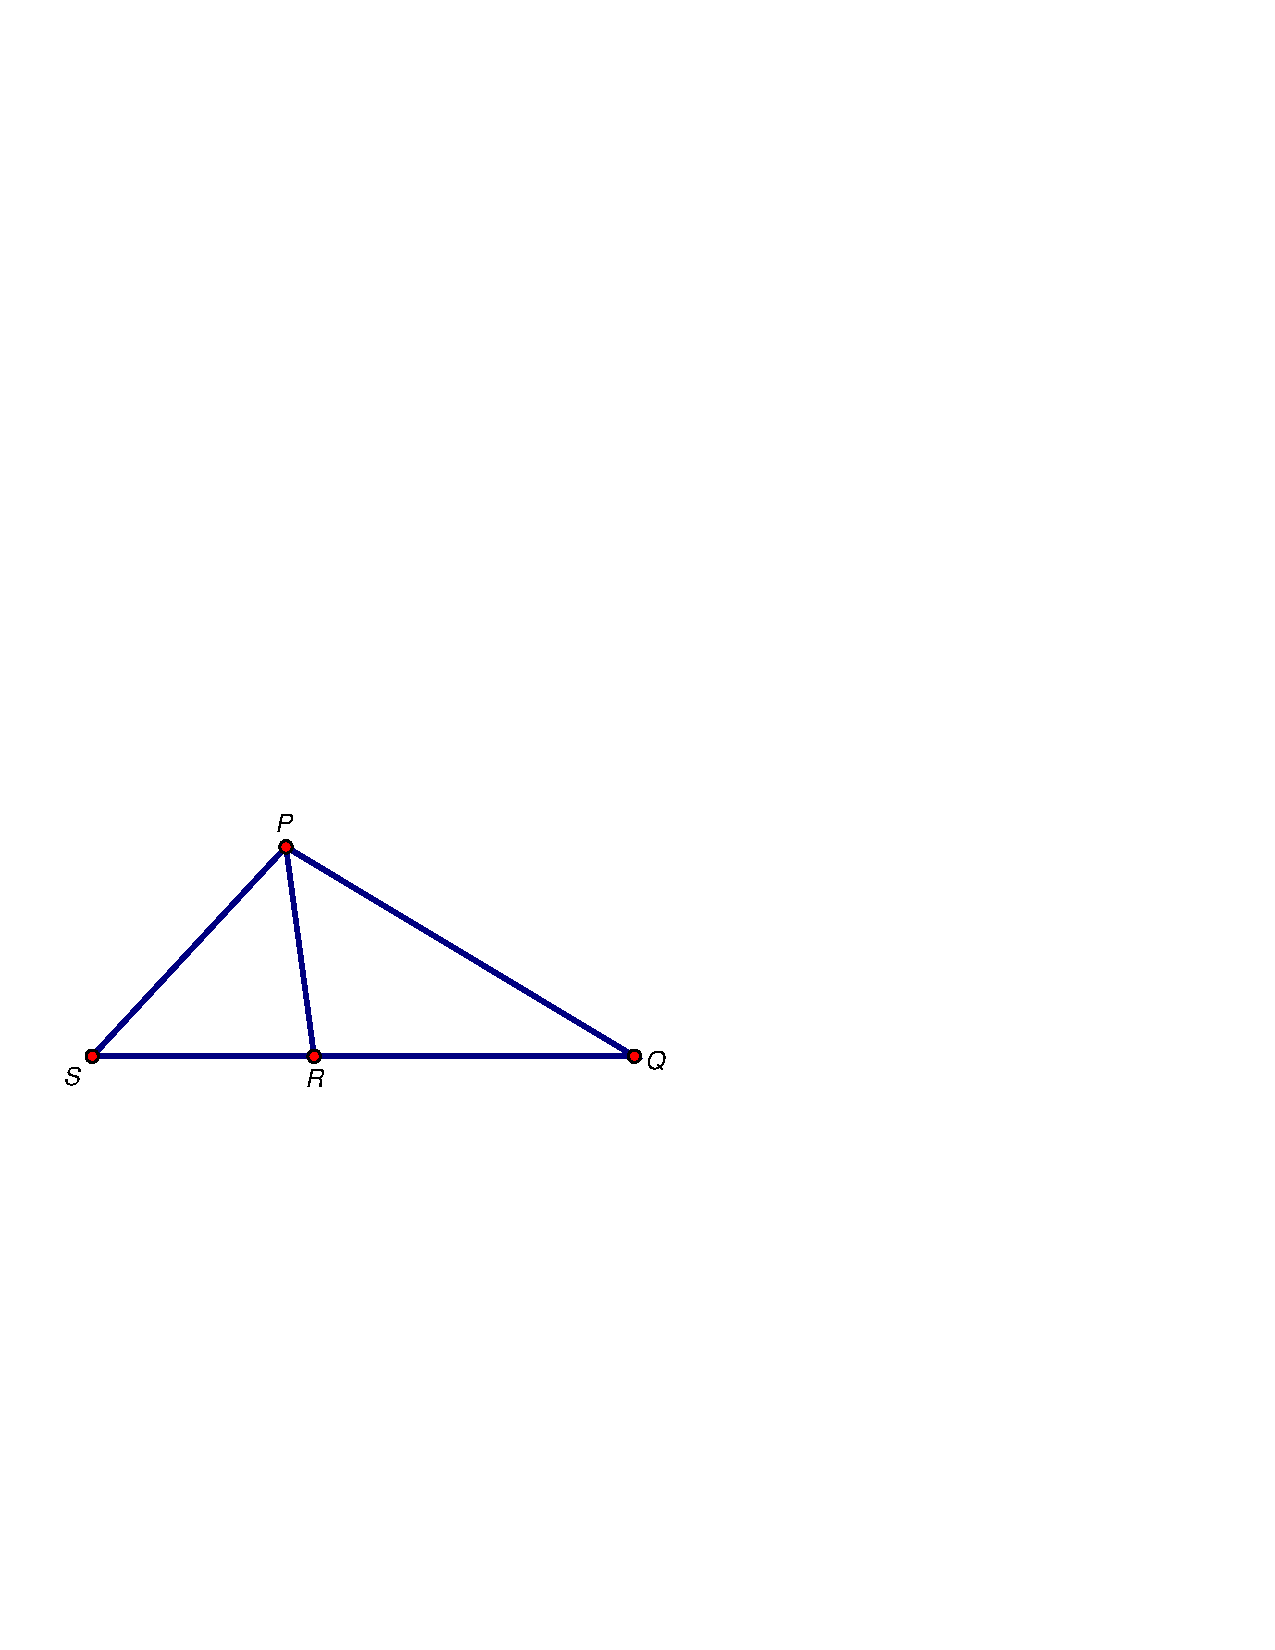
\includegraphics[scale=0.5]{SideSplitter1}$$
\end{prob}

\begin{prob}
For the trapezoid below, explain why the area of $\triangle BAD$ is equal to the area of $\triangle BAC$.  Name two other triangles that have the same area.
$$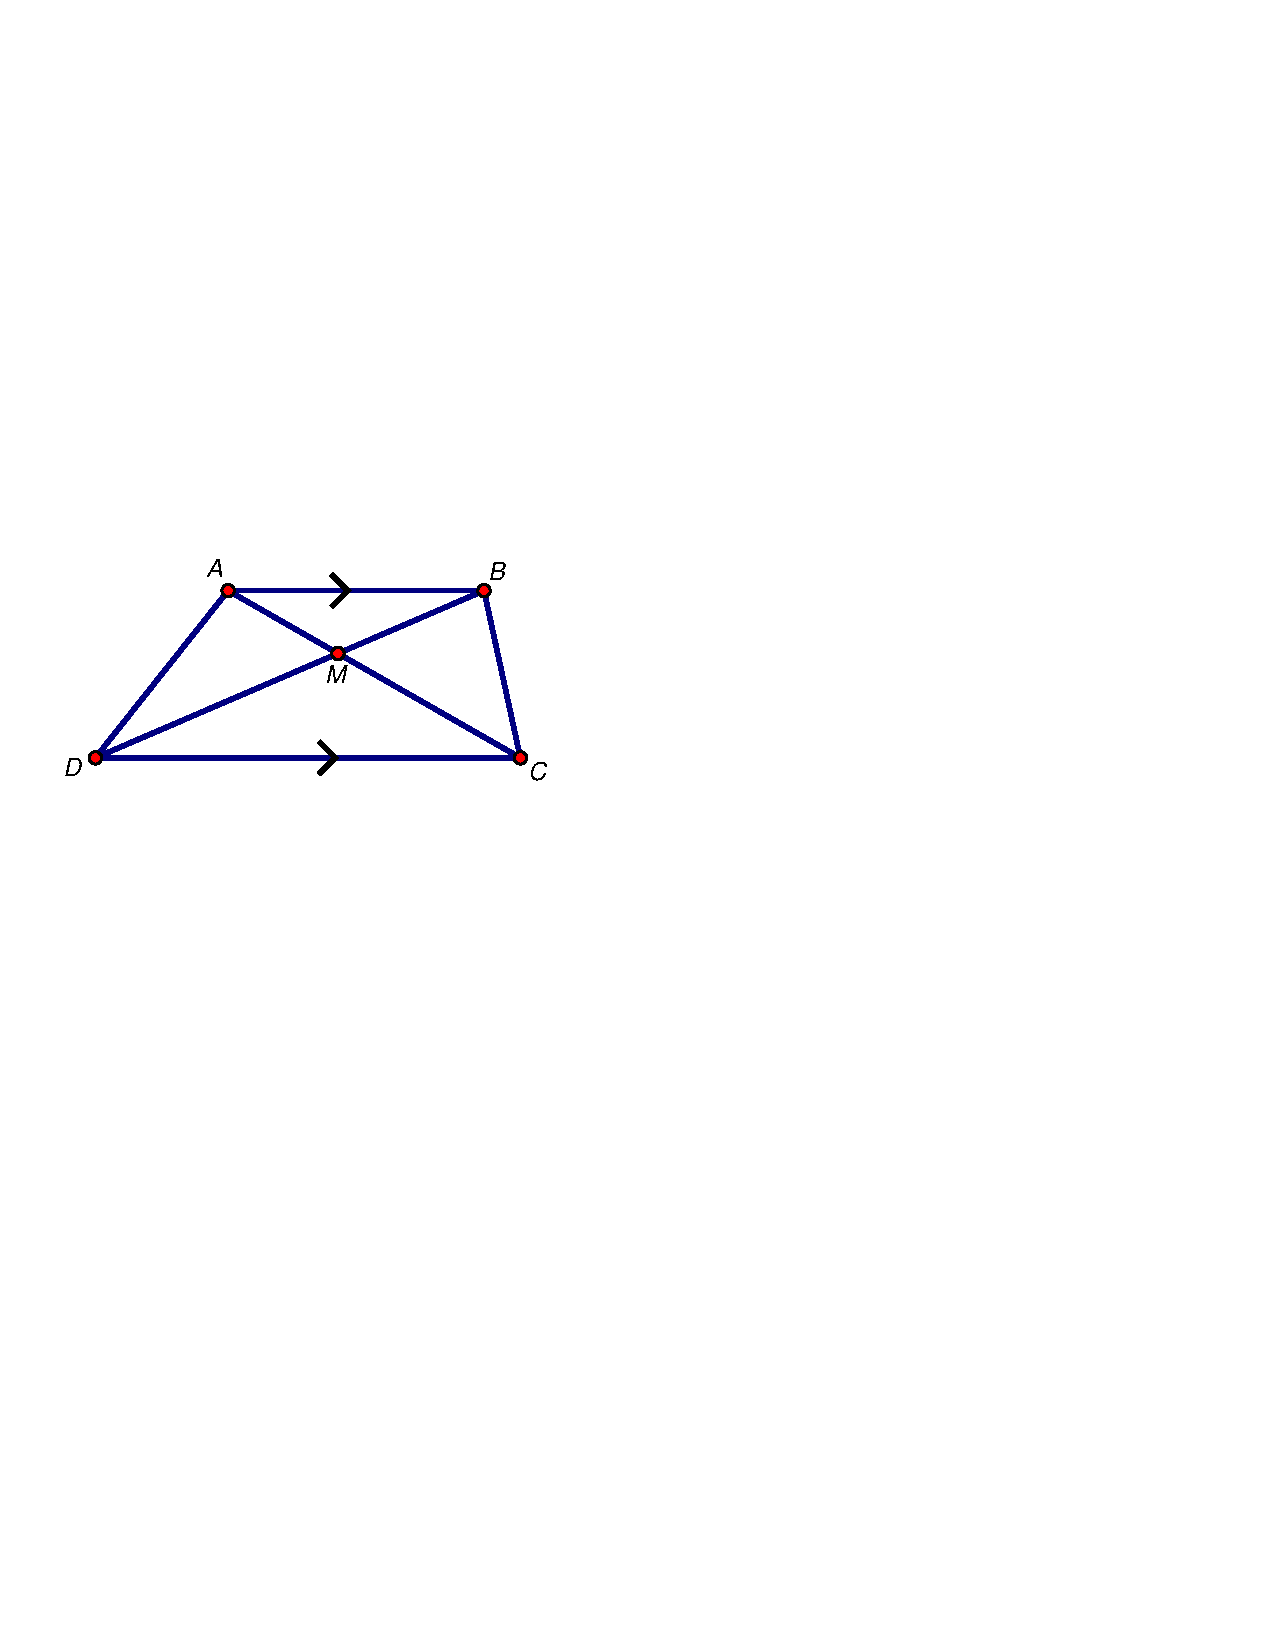
\includegraphics[scale=0.5]{SideSplitter2}$$
\end{prob}

\begin{prob}
For the parallelogram below, which triangle has the greatest area: $\triangle XYZ$, $\triangle WXY$, $\triangle ZWX$, or $\triangle YZW$?  Explain.  
$$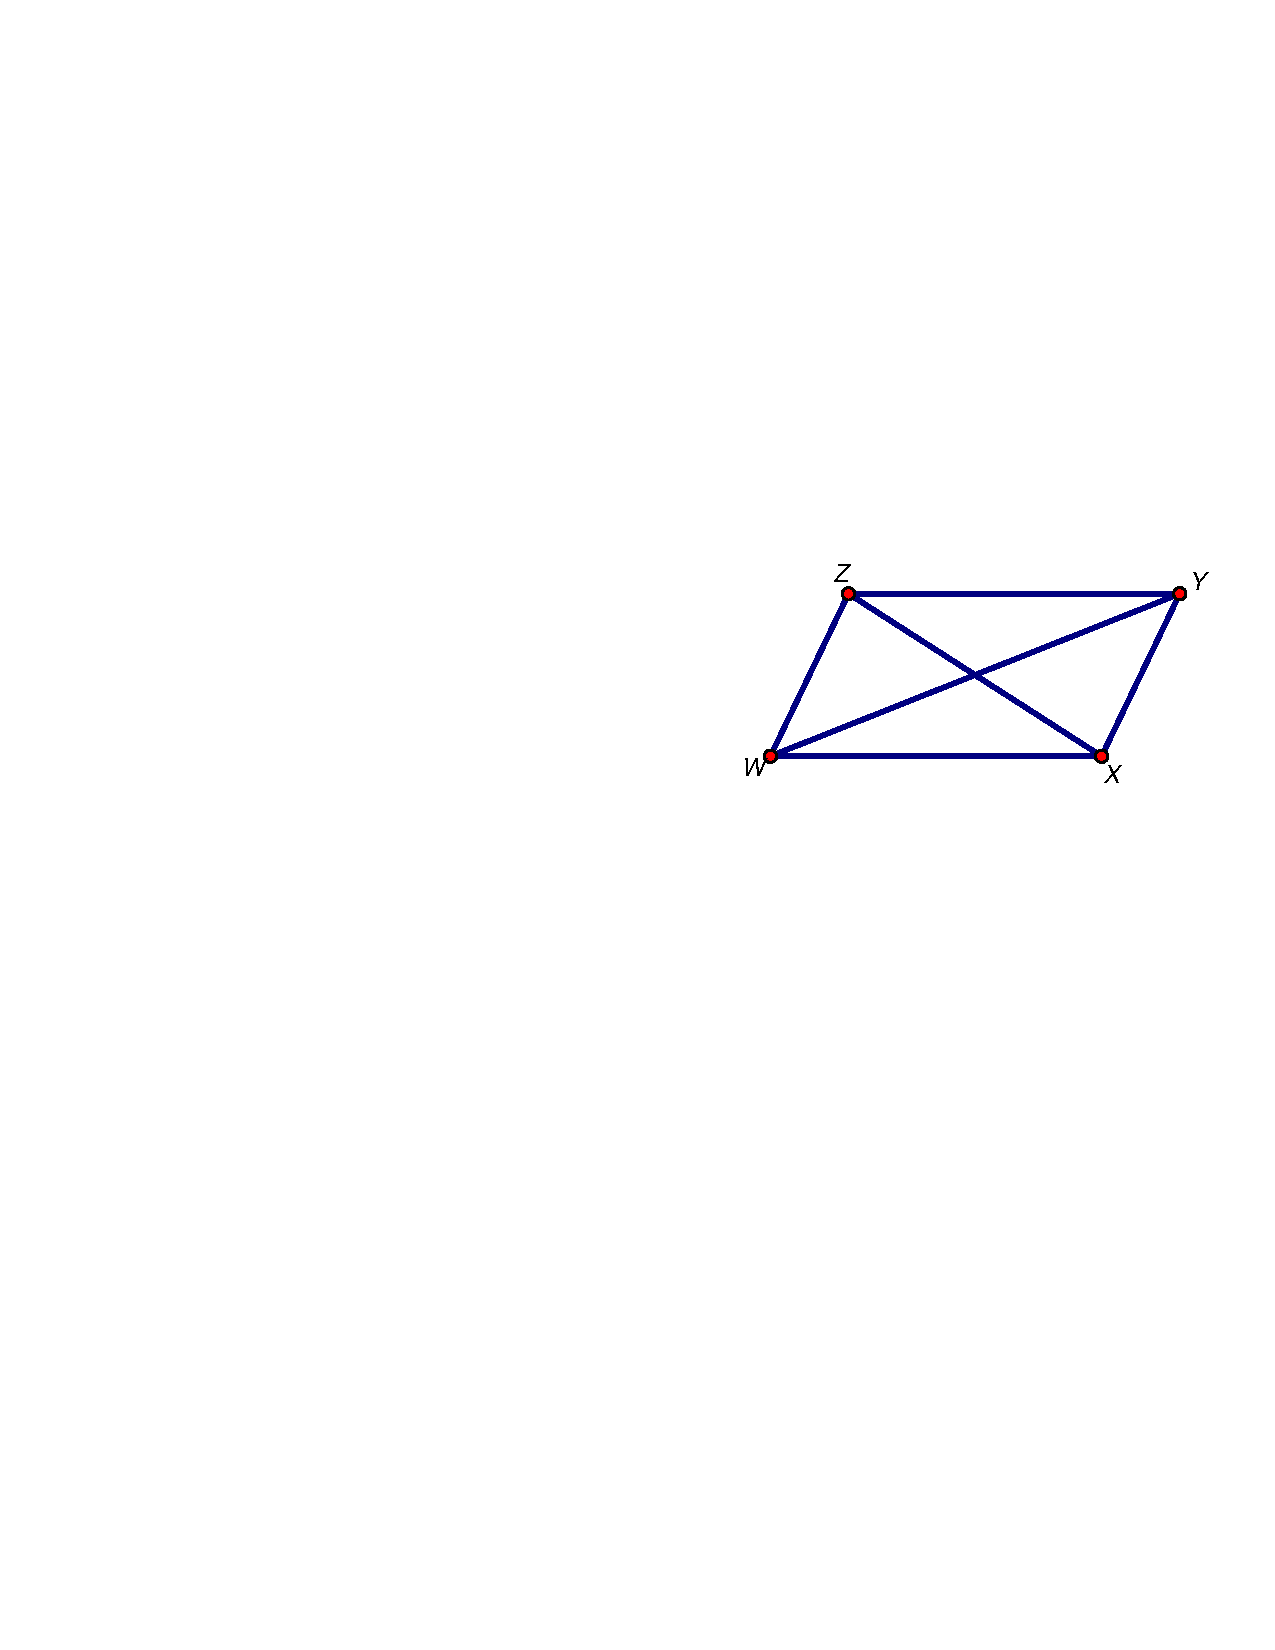
\includegraphics[scale=0.5]{SideSplitter3}$$
\end{prob}

\begin{prob}
Prove:  If a line in a triangle is parallel to a side of a triangle, then it splits the other sides of the triangle proportionally.
$$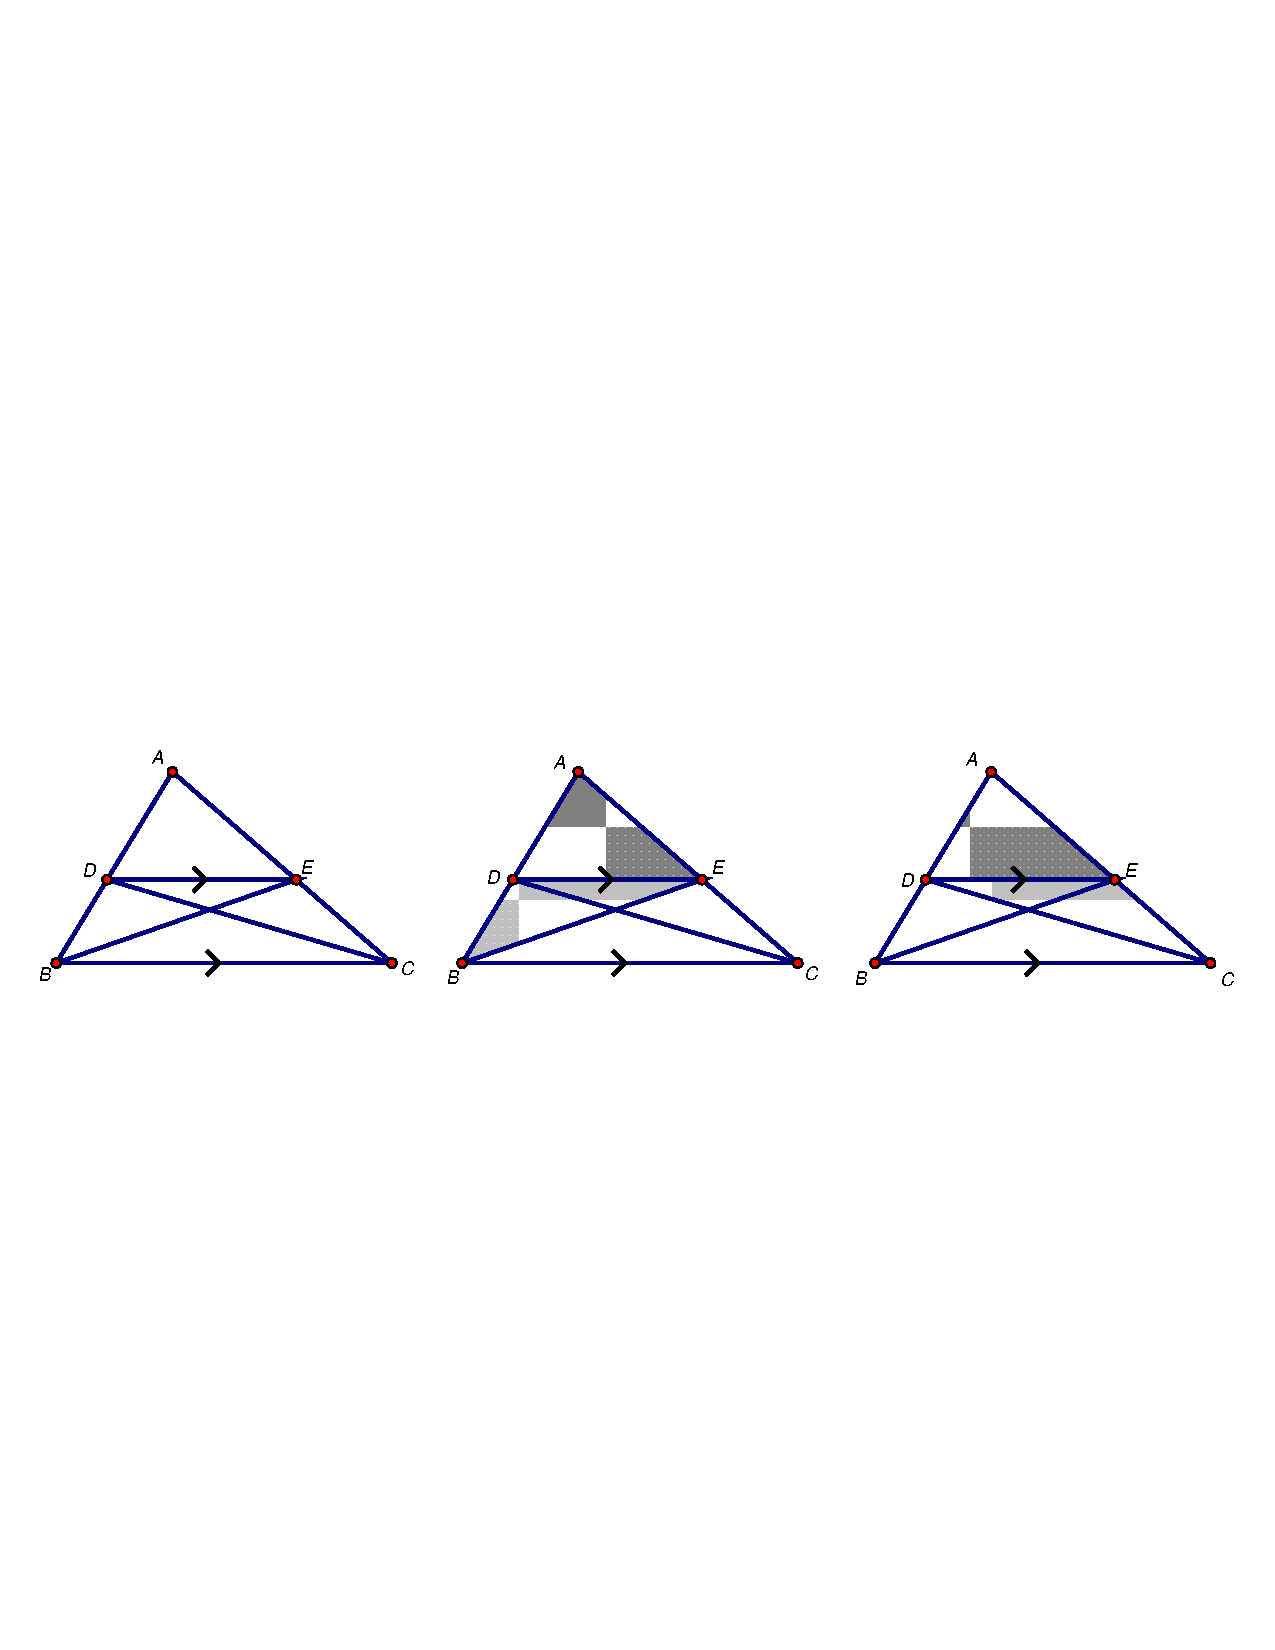
\includegraphics[scale=0.7]{SideSplitter}$$
\begin{enumerate}
\item How do the areas of $\triangle ADE$ and $\triangle DBE$ relate to $AD$ and $DB$?  Explain.  
\item How do the areas of $\triangle ADE$ and $\triangle CED$ relate to $AE$ and $CE$?  Explain. 
\item How do the areas of $\triangle BDE$ and $\triangle CED$ compare?  Explain.  
\item Use the previous results to show that $\frac{AD}{DB} = \frac{AE}{EC}$.  
\item Where in the proof did you use the fact that $\overline{DE} \parallel \overline{BC}$?  
\end{enumerate}
\end{prob}

\begin{prob}
Prove:  In the previous figure, $\frac{AB}{AD} = \frac{AC}{AE} = \frac{BC}{DE}$.  
\begin{enumerate}
\item Use the results of the previous problem and some algebra to show that $\frac{AB}{AD} = \frac{AC}{AE}$
\item How do we know that $\angle ADE \cong \angle ABC$?  
\item Translate $\triangle ADE$ by the vector $\overrightarrow{DB}$ so that the image $\angle A'D'E'$ of $\angle ADE$ coincides with $\angle ABC$.  Draw a picture of the result.  
\item What segments are parallel now?  How do you know?  
\item Now explain why $\frac{BC}{DE}$ is equal to the common ratio in part (a).  
\end{enumerate}
\end{prob}

\begin{prob}
Prove:  If a line in a triangle splits two sides proportionally, then it is parallel to the third side of the triangle.  (Hint:  Using the previous figures, draw a line through $D$ and parallel to $\overline{BC}$, and let $X$ be the point where the new line intersects $\overline{AC}$.  By the previous results, $\overline{DX}$ divides the sides proportionally.  Then argue that $E$ and $X$ must be the same point.)  
\end{prob}


